\documentclass[fleqn, a4paper, 12pt]{article}
\usepackage{amsmath, amssymb, amsthm}
\usepackage{gensymb}
\usepackage{commath}
\usepackage{xcolor}
\usepackage{cancel}
\usepackage{siunitx}
\usepackage{tikz, pgfplots}
	\usetikzlibrary{calc, hobby, patterns, intersections}
\usepackage{graphicx}
\usepackage{hyperref}
\usepackage{datetime}
\usepackage{ulem}
\usepackage{xfrac}
\usepackage{asymptote}
\usepackage{enumerate}
\setcounter{secnumdepth}{4}
\newcommand\numberthis{\addtocounter{equation}{1}\tag{\theequation}}

\newcommand{\AxisRotator}[1][rotate=0]{%
	\tikz [x=0.25cm,y=0.60cm,line width=.2ex,-stealth,#1] \draw (0,0) arc (-150:150:1 and 1);%
}

\theoremstyle{definition}
\newtheorem{example}{Example}
\newtheorem{definition}{Definition}

\theoremstyle{theorem}
\newtheorem{theorem}{Theorem}

\newenvironment{solution}
{\begin{proof}[Solution]\let\qed\relax}
	{\end{proof}}

\newcommand{\curl}{\mathrm{curl\,}}

%\renewcommand{\int_{min}^{max}}{\int\displaylimits_{min}^{max}}

%opening
\title{Lecture 20}
\author{Aakash Jog}
\date{\formatdate{6}{1}{2015}}

\begin{document}

\maketitle
%\setlength{\mathindent}{0pt}

\tableofcontents

\newpage
\section{Simple Harmonic Oscillators}

\begin{align*}
	\ddot{x} + {\omega_0}^2 x &= 0\\
	\therefore x &= \widetilde{A} \cos \omega_0 t + \widetilde{B} \sin \omega_0 t\\
	&= A \sin (\omega_0 t + \varphi)
\end{align*}

\begin{example}
	A simple pendulum with with length $l$ and mass $m$ attached at its end is oscillating under gravity. Find its angular frequency.
\end{example}

\begin{solution}[Solution using force dynamics]
	\hspace{1cm}\\
	\begin{tikzpicture}
		\def\angle{30};
		\def\l{4};
		\def\F{1};
	
		\coordinate (pendulum top) at (0,0);
		\coordinate (pendulum bottom) at ({270-\angle}:\l);
	
		\draw (pendulum top) -- (pendulum bottom);
		\fill (pendulum bottom) circle [radius = 3pt] node [below left] {$m$};
		
		\draw [dashed] (pendulum top) -- (-90:\l);
		
		\node at ({270-(\angle/2)}:1) {$\theta$};
		
		\draw [dashed] (pendulum bottom) arc ({270-\angle}:{270+\angle}:\l);
		
		%forces
		\draw [-stealth, red] (pendulum bottom) -- ++({90-\angle}:\F) node [left] {$T$};
		\draw [-stealth, red] (pendulum bottom) -- ++(-90:\F) node [left] {$mg$};
	\end{tikzpicture}
	\begin{align*}
		m l \ddot{\theta} &= - m g \sin \theta\\
		\therefore \ddot{\theta} + \dfrac{g}{l} \sin \theta &= 0\\
		\intertext{If $\theta$ is very small, $\sin \theta \approx \theta$}
		\therefore \ddot{\theta} + \dfrac{g}{l} \theta &= 0\\
		\therefore \omega &= \sqrt{\dfrac{g}{l}}
	\end{align*}
\end{solution}

\begin{solution}[Solution using conservation of energy]
	\hspace{1cm}\\
	\begin{tikzpicture}
		\def\angle{30};
		\def\l{4};
		\def\F{1};
		
		\coordinate (pendulum top) at (0,0);
		\coordinate (pendulum bottom) at ({270-\angle}:\l);
		
		\draw (pendulum top) -- (pendulum bottom);
		\fill (pendulum bottom) circle [radius = 3pt] node [below left] {$m$};
		
		\draw [dashed] (pendulum top) -- (-90:\l);
		
		\node at ({270-(\angle/2)}:1) {$\theta$};
		
		\draw [dashed] (pendulum bottom) arc ({270-\angle}:{270+\angle}:\l);
		
		%forces
		\draw [-stealth, red] (pendulum bottom) -- ++({90-\angle}:\F) node [left] {$T$};
		\draw [-stealth, red] (pendulum bottom) -- ++(-90:\F) node [left] {$mg$};
	\end{tikzpicture}
	\begin{align*}
		E &= \dfrac{1}{2} m (l \dot{\theta})^2 + m g l(1 - \cos \theta)\\
		\therefore \dot{E} &= m l^2 \dot{\theta} \ddot{\theta} + m g l \dot{\theta} \sin \theta\\
		\intertext{If $\theta$ is very small, $\sin \theta \approx \theta$}
		\therefore &= m l^2 \dot{\theta} \ddot{\theta} + m g l \dot{\theta} \theta\\
		\therefore &= l \ddot{\theta} + g \theta\\
		\therefore &= \ddot{\theta} + \dfrac{g}{l} \theta\\
		\therefore \omega &= \sqrt{\dfrac{g}{l}}
	\end{align*}
\end{solution}

\begin{tikzpicture}
	
\end{tikzpicture}

\subsection{Analysis of Potential Energy}

Let $\xi = x_0 - x$.\\
By Taylor's expansion of $U(x)$,
\begin{align*}
	U(x) &= U(x_0) + \cancelto{0}{U'(x_0)} (x - x_0) + \dfrac{U''(x_0)}{2} (x - x_0)^2\\
	\therefore U(\xi) &= U(x_0) + \dfrac{1}{2} U''(x_0) \xi^2\\
	\therefore \omega &= \sqrt{\dfrac{U''(x_0)}{``m"}}
\end{align*}
\begin{align*}
	E &= \dfrac{1}{2} ``m" (\dot{x})^2 + U(x)\\
	&= \dfrac{1}{2} ``m" (\dot{x})^2 + U(x_0) + \dfrac{1}{2} U''(x_0) \xi^2\\
	&= \dfrac{1}{2} ``m" (\dot{\xi})^2 + U(x_0) + \dfrac{1}{2} U''(x_0) \xi^2\\
	\therefore \dot{E} &= \dot{\xi} ``m" \left( \ddot{\xi} + \dfrac{U''(x_0)}{``m"} \xi \right)\\
	\therefore 0 &= \ddot{\xi} + \dfrac{U''(x_0)}{``m"} \xi\\
	\therefore \omega &= \sqrt{\dfrac{U''(x_0)}{``m"}}
\end{align*}



\begin{example}
	A particle of mass $m$ is dropped from a height $h$ above a spring of natural length $l$. Find angular frequency of the oscillations of the system.
\end{example}

\begin{solution}
	\hspace{1cm}\\
	\begin{tikzpicture}
		\def\l{4};
		\def\x{0};
		\def\h{2};
		\def\segmentlength{4}

		\coordinate (spring bottom) at (0,0);
		\coordinate (spring top) at (0,{\l + \x});
		\coordinate (initial position) at (0,{\l + \h});

		\draw [decorate, decoration = {coil, segment length = {(\l + \x)/(\l)*\segmentlength}}] (spring bottom) -- (spring top);
		\fill (initial position) circle [radius = 2pt];
		
		\draw (-1,0) -- (1,0);
	\end{tikzpicture}
	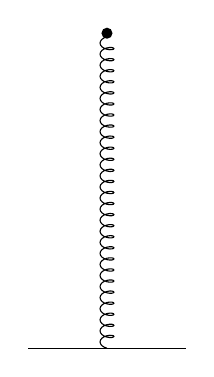
\begin{tikzpicture}
		\def\l{4};
		\def\x{0};
		\def\h{2};
		\def\segmentlength{4}
		
		\coordinate (spring bottom) at (0,0);
		\coordinate (spring top) at (0,{\l + \x});
		\coordinate (initial position) at (0,{\l + \h});
		
		\draw [decorate, decoration = {coil, segment length = {(\l + \x)/(\l)*\segmentlength}}] (spring bottom) -- (spring top);
		\fill (spring top) circle [radius = 2pt];
		
		\draw (-1,0) -- (1,0);
	\end{tikzpicture}
	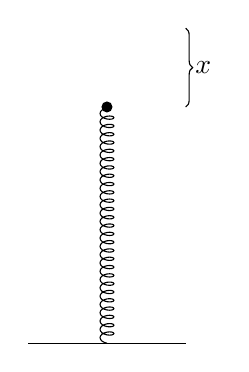
\begin{tikzpicture}
		\def\l{4};
		\def\x{-1};
		\def\h{2};
		\def\segmentlength{4}
		
		\coordinate (spring bottom) at (0,0);
		\coordinate (spring top) at (0,{\l + \x});
		\coordinate (initial position) at (0,{\l + \h});
		
		\draw [decorate, decoration = {coil, segment length = {(\l + \x)/(\l)*\segmentlength}}] (spring bottom) -- (spring top);
		\fill (spring top) circle [radius = 2pt];
		
		\draw [decorate, decoration = brace] ($ (0,\l) + (1,0) $) -- ($ (spring top) + (1,0) $) node [midway, right] {$x$};
		
		\draw (-1,0) -- (1,0);
	\end{tikzpicture}\\
	\begin{align*}
		E &= \dfrac{1}{2} m (\dot{x})^2 + \dfrac{1}{2} k x^2 - m g x\\
		U(x) &= \dfrac{1}{2} k x^2 - m g x\\
		\therefore U'(x_0) &= k x_0 - m g\\
		\therefore 0 &= k x_0 - m g\\
		\therefore k x_0 &= m g\\
		\therefore x_0 &= \dfrac{m g }{k}\\
		\therefore U'' (x_0) &= k\\
		&> 0\\
		\therefore U(x) &= U(x_0) + \dfrac{1}{2} k \left( x - \dfrac{m g}{k} \right)^2
		\intertext{Let $\xi = x - \dfrac{m g}{k}$}
		\therefore E &= \dfrac{1}{2} m (\dot{\xi})^2 + \dfrac{1}{2} k \xi^2 + U(x_0)\\
		\therefore \xi^2 + \dfrac{k}{m} \xi &= 0\\
		\therefore \omega &= \sqrt{\dfrac{k}{m}}
	\end{align*}
\end{solution}

\begin{example}
	A body of volume $V$ and volume density $\rho$ is immersed in a fluid of volume density $\rho_0$. It floats with some portion above the surface. It is perturbed from its equilibrium position.
\end{example}

\begin{solution}
	\hspace{1cm}\\
	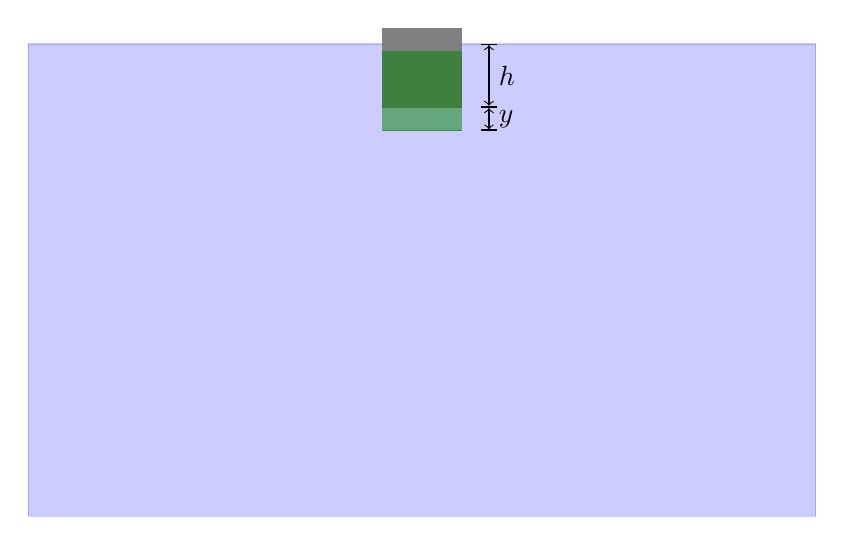
\begin{tikzpicture}
		\def\l{10};
		\def\d{6};
		\def\a{1};
		\def\h{0.8};
		\def\y{0.3};
		
		\filldraw [blue, opacity = 0.2] ({-\l/2},0) rectangle ({\l/2},{-\d});
		
		\filldraw [gray] ({-\a/2},{\a - \h}) rectangle ({\a/2},{-\h});
		
		\draw [|<->|, xshift = 10] ({\a/2},{-\h}) -- ({\a/2},0) node [midway, right] {$h$};
		
		\filldraw [green!50!black, opacity = 0.5] ({-\a/2},{\a - \h - \y}) rectangle ({\a/2},{-\h - \y});
		
		\draw [|<->|, xshift = 10] ({\a/2},{-\h - \y}) -- ({\a/2}, {-\h}) node [midway, right] {$y$};
	\end{tikzpicture}\\
	When the body is in equilibrium, let the height of the submerged portion be $h$. Therefore,
	\begin{align*}
		\rho_0 a^2 h g &= \rho a^3 g\\
		\therefore h &= \dfrac{\rho}{\rho_0} a
	\end{align*}
	After the body is pushed down by a small distance $y$,
	\begin{align*}
		\rho a^3 \ddot{y} &= \rho a^3 g - \rho_0 (h + y) a^2 g\\
		&= \cancel{\rho a^3 g} - \cancel{\rho_0 h a^2 g} - \rho_0 y a^2 g\\
		\therefore \rho a^3 \ddot{y} &= - \rho_0 a^2 g y\\
		\therefore \ddot{y} + \dfrac{\rho_0}{\rho} \cdot \dfrac{g}{a} \cdot y &= 0\\
		\therefore {\omega_0}^2 &= \dfrac{\rho_0}{\rho} \cdot \dfrac{g}{a}
	\end{align*}
\end{solution}

\begin{example}
	Find the angular frequency of the oscillations and the maximal $A$ such that the string does not slack.\\
	\begin{tikzpicture}
		\def\R{2};
		\def\h{6}
		\def\springlength{3};
		\def\segmentlength{4};
		\def\l{3};
		\def\A{2};
		\def\x{0};
		\def\F{1};
		\def\xo{1};
		
		\coordinate (pulley centre) at (\R,\h);
		\coordinate (pulley left) at ($ (pulley centre) + (180:\R) $);
		\coordinate (pulley right) at ($ (pulley centre) + (0:\R) $);
		\coordinate (m1) at ($ (pulley right) + (-90:\l) $);
		\coordinate (spring bottom) at (0,0);
		\coordinate (spring top) at ($ (spring bottom) + (90:\springlength) $);
		
		\draw ($ (spring bottom) + (-1,0) $) -- ($ (spring bottom) + (1,0) $);
		
		\draw [decorate, decoration = {coil, segment length = {(\springlength + \x)/(\springlength)*\segmentlength}}] (spring bottom) -- (spring top);
		\draw (spring top) -- (pulley left);
		
		\draw (pulley centre) -- ++(90:{2*\R});
			\draw ($ (pulley centre) + (90:{2*\R}) + (-1,0) $) -- ($ (pulley centre) + (90:{2*\R}) + (1,0) $);
		\draw (pulley centre) circle [radius = \R] node [below] {$m_2$};
		
		\draw (pulley right) -- (m1);
		\fill (m1) circle [radius = 2pt] node [right] {$m_1$};
		
		\draw [dashed] (m1) -- ++(-90:\A);
		\fill ($ (m1) + (-90:\A) $)circle [radius = 2pt];
		
		\draw [|-stealth] ($ (m1) + (1,0)$) -- ++(-90:\A) node [midway, right] {$A$};
	\end{tikzpicture}
\end{example}

\begin{solution}
	Let $x_0$ be the extension of the spring at equilibrium.\\
	\begin{tikzpicture}
		\def\R{2};
		\def\h{6}
		\def\springlength{3};
		\def\segmentlength{4};
		\def\l{3};
		\def\A{2};
		\def\x{0};
		\def\F{1};
		\def\xo{1};
		
		\coordinate (pulley centre) at (\R,\h);
		\coordinate (pulley left) at ($ (pulley centre) + (180:\R) $);
		\coordinate (pulley right) at ($ (pulley centre) + (0:\R) $);
		\coordinate (m1) at ($ (pulley right) + (-90:\l) $);
		\coordinate (spring bottom) at (0,0);
		\coordinate (spring top) at ($ (spring bottom) + (90:\springlength) $);
		
		\draw ($ (spring bottom) + (-1,0) $) -- ($ (spring bottom) + (1,0) $);
		
		\draw [decorate, decoration = {coil, segment length = {(\springlength + \x)/(\springlength)*\segmentlength}}] (spring bottom) -- (spring top);
		\draw (spring top) -- (pulley left);
		
		\draw (pulley centre) -- ++(90:{2*\R});
		\draw ($ (pulley centre) + (90:{2*\R}) + (-1,0) $) -- ($ (pulley centre) + (90:{2*\R}) + (1,0) $);
		\draw (pulley centre) circle [radius = \R] node [right] {$m_2g$};
		
		\draw (pulley right) -- (m1);
		\fill (m1) circle [radius = 2pt] node [right] {$m_1$};
		
		\draw [dashed] (m1) -- ++(-90:\A);
		\fill ($ (m1) + (-90:\A) $)circle [radius = 2pt];
		
		\draw [|-stealth] ($ (m1) + (1,0)$) -- ++(-90:\A) node [midway, right] {$A$};
		
		\draw [stealth-|] ($ (spring top) + (-1,0) $) -- ++(-90:\xo) node [midway, left] {$x_0$};
		
		%forces
		\draw [-stealth, green] (spring top) -- ++(-90:\F) node [right] {$k x_0$};
		\draw [-stealth, green] (spring top) -- ++(90:\F) node [right] {$T_2$};
	
		\draw [-stealth, blue] (pulley centre) -- ++(-90:\F) node [right] {$m_2$};
		\draw [-stealth, blue] (pulley centre) -- ++(90:\F) node [right] {$T_3$};
		\draw [-stealth, blue] (pulley left) -- ++(-90:\F) node [right] {$T_2$};
		\draw [-stealth, blue] (pulley right) -- ++(-90:\F) node [right] {$T_1$};
	
		\draw [-stealth, red] (m1) -- ++(-90:\F) node [right] {$m_1 g$};
		\draw [-stealth, red] (m1) -- ++(90:\F) node [right] {$T_1$};
	\end{tikzpicture}\\
	Therefore, at equilibrium,
	\begin{align*}
		T_2 &= k x_0\\
		T_1 &= m_1 g\\
		T_1 &= T_2
	\end{align*}
	Therefore,
	\begin{align*}
		m_1 g &= k x_0
	\end{align*}
	When $m_1$ is pulled down some $x$,
	\begin{align*}
		T_2 &= k (x_0 + x)\\
		m_1 \ddot{x} &= m_1 g - T_1\\
		T_1 R - T_2 R &= \dfrac{1}{2} m_2 R^2 \alpha_2\\
		&= \dfrac{1}{2} m_2 R \ddot{x}\\
		\therefore T_1 - T_2 &= \dfrac{1}{2} m_2 \ddot{x}\\
		\therefore -m_1 \ddot{x} + m_1 g - k (x_0 + x) &= \dfrac{1}{2} m_2 \ddot{x}
	\end{align*}
	Solving, 
	\begin{align*}
		\omega &= \sqrt{\dfrac{k}{m_1 + \sfrac{1}{2} \cdot m_2}}
	\end{align*}
	For the string to never slack, $T_1 > 0$ and $T_2 > 0$. Therefore,
	\begin{align*}
		m_1 g - m_2 \ddot{x} &> 0\\
		\therefore m_1 g - m_1 A \omega^2 \cos \omega t &> 0
	\end{align*}
	\begin{align*}
		k x_0 + k x &> 0\\
		\therefore m_1 g + k A \cos \omega t &> 0
	\end{align*}
	Solving, 
	\begin{align*}
		A &\leq \dfrac{m_1 g}{k}\\
		\intertext{and}
		A &\leq \dfrac{g \left( m_1 + \sfrac{1}{2} \cdot m_2 \right)}{k}
	\end{align*}
	Therefore,
	\begin{align*}
		A_{\text{max}} &= \dfrac{m_1 g}{k}
	\end{align*}
\end{solution}

\begin{example}
	Let a rigid body of mass $m$ be pivoted at a point at a distance $d$ from its centre of mass. Let the moment of inertia of the body about the axis be $I_0$. Find the angular frequency of its oscillations.
\end{example}

\begin{solution}
	Let the angle between the line joining the centre of mass and the pivot point, and the vertical be $\theta$.
	\begin{align*}
		I_0 \ddot{\theta} &= - d \cdot m g \cdot \sin \theta\\
		\therefore \ddot{\theta} + \dfrac{d m g}{I_0} \sin \theta &= 0\\
		\intertext{If $\theta$ is very small, $\sin \theta \approx \theta$}
		\therefore \ddot{\theta} + \dfrac{d m g}{I_0} \theta &= 0\\
		\therefore \omega &= \sqrt{\dfrac{d m g}{I_0}}
	\end{align*}
\end{solution}

\begin{example}
	A rod of mass $m$ and length $L$ has a particle of mass $m$ attached at its bottom. It has a loop at its top through which a string is threaded. A force $F$ is acting on it, for time $\Delta t$, at $h$ from the top. Find $h$ such that the top of the rod does not move.\\
	\begin{tikzpicture}
		\def\L{4};
		\def\r{2pt};
		\def\h{8/9*\L};
		\def\F{1};
		
		\coordinate (rod top) at ($ (0,0) + (-90:\r) $);
		\coordinate (rod bottom) at ($ (rod top) + (-90:\L) $);
		
		\draw (0,0) circle [y radius = \r, x radius = {0.8*\r}];
		
		\draw (-\L,0) -- (\L,0);
		
		\draw (rod top) -- (rod bottom);
		\fill (rod bottom) circle [radius = 2pt] node [right] {$m$};
		
		\draw [stealth-] (0,-\h) -- ++(0:\F) node [right] {$F$};
		
		\draw [xshift = -10, |<->|] (0,0) -- (-90:\h) node [midway, fill = white] {$h$};
	\end{tikzpicture}
\end{example}

\begin{solution}
	Let $d$ be the distance between the top and the centre of mass.
	\begin{align*}
		d &= \dfrac{\dfrac{L}{2} m + L m}{2 m}\\
		&= \dfrac{3}{4} L\\
		I_{\text{top}} &= \dfrac{4}{3} m L^2\\
		\omega^2 &= \dfrac{d m g}{L}\\
		\therefore \omega^2 &= \dfrac{9}{8} \cdot \dfrac{g}{L}
	\end{align*}
	For the top of the rod to be stationary,
	\begin{align*}
		h F \Delta t &= I_{\text{top}} \omega\\
		\therefore h F \Delta t &= \dfrac{4}{3} m L^2 \omega\\
		\therefore \omega &= \dfrac{3 h F \Delta t}{4 m L^2}
	\end{align*}
	and
	\begin{align*}
		v_{\text{COM}} &= \omega d\\
		\therefore v_{\text{COM}} &= \dfrac{F \Delta t}{2 m}
	\end{align*}
	Therefore,
	\begin{align*}
		h &= \dfrac{8}{9} L
	\end{align*}
\end{solution}

\section{Damped Oscillations}

A spring mass oscillator is submerged in water such that the friction between the mass and the water is
\begin{align*}
	\overrightarrow{f} &= - \beta \overrightarrow{v}
\end{align*}\\
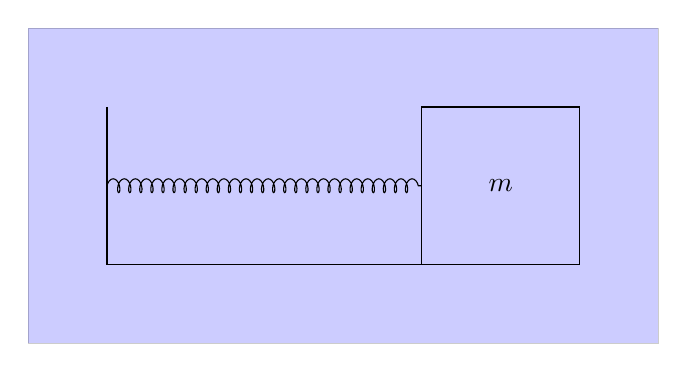
\begin{tikzpicture}
	\def\l{4};
	\def\x{1};
	\def\segmentlength{4};
	
	\filldraw [fill = blue, opacity = 0.2] (-1,3) rectangle ({\l + 2 + 1},-1);
	
	\draw (0,2) -- (0,0) -- (\l,0);
	
	\draw [decorate, decoration = {coil, segment length = \segmentlength}](0,1) -- (\l,1);
	
	\draw (\l,2) rectangle  node {$m$} ({\l + 2}, 0);
\end{tikzpicture}
Therefore, 
\begin{align*}
	m \ddot{x} &= - k x - \beta \dot{x}\\
	\therefore \ddot{x} + \dfrac{\beta}{m} \dot{x} + \dfrac{k}{m} x &= 0\\
	\therefore \ddot{x} + \dfrac{\beta}{m} \dot{x} + {\omega_0}^2 x &= 0	
\end{align*}
Therefore, the characteristic equation is
\begin{align*}
	\lambda^2 + \dfrac{\beta}{m} \lambda + {\omega_0}^2 &= 0
\end{align*}
\begin{align*}
	\therefore \lambda &= \dfrac{-\dfrac{\beta}{m} \pm \sqrt{\dfrac{\beta^2}{m^2} - 4 {\omega_0}^2}}{2}\\
	&= -\dfrac{\beta}{2m} \pm \sqrt{\left( \dfrac{\beta}{2m} \right)^2 - {\omega_0}^2}
\end{align*}

\begin{tabular}{c c}
	Strong damping & $\dfrac{\beta}{2m} > \omega_0$\\[2ex]
	Critical damping & $\dfrac{\beta}{2m} = \omega_0$\\[2ex]
	Weak damping & $\dfrac{\beta}{2m} < \omega_0$\\[2ex]
\end{tabular}\\
Oscillations occur in case of weak damping.\\
Therefore,
\begin{align*}
	\lambda &= -\dfrac{\beta}{2m} \pm i \sqrt{{\omega_0}^2 - \left( \dfrac{\beta}{2m} \right)^2}\\
	\intertext{Let $\omega_1 = \sqrt{{\omega_0}^2 - \left( \dfrac{\beta}{2m} \right)^2}$}
	\therefore x &= e^{-\sfrac{\beta}{2m} \cdot t} \left( \widetilde{A} \cos \omega_1 t + \widetilde{B} \sin \omega_1 t \right)
\end{align*}
Let
\begin{align*}
	x(t = 0) &= 0\\
	\dot{x}(t = 0) &= v_0
\end{align*}
Solving,
\begin{align*}
	\widetilde{A} &= 0\\
	\widetilde{B} &= \dfrac{v_0}{\omega_1}
\end{align*}
Therefore,
\begin{align*}	
	x(t) &= \dfrac{v_0}{\omega_1} e^{-\sfrac{\beta}{2m} \cdot t} \sin \omega_1 t\\
	x(t) &= \dfrac{v_0}{\sqrt{{\omega_0}^2 - \left( \dfrac{\beta}{2m} \right)^2}} e^{-\sfrac{\beta}{2m} \cdot t} \sin \left( \sqrt{{\omega_0}^2 - \left( \dfrac{\beta}{2m} \right)^2} t \right)
\end{align*}

In case of critical damping,
\begin{align*}
	x &= e^{-\sfrac{\beta}{2m} \cdot t} (\widetilde{A} + \widetilde{B} t)
\end{align*}
Let
\begin{align*}
	x(t = 0) &= 0\\
	\dot{x}(t = 0) &= v_0
\end{align*}
Solving,
\begin{align*}
	\widetilde{A} &= 0\\
	\widetilde{B} &= v_0
\end{align*}
Therefore,
\begin{align*}
	x &= v_0 t e^{-\sfrac{\beta}{2m} \cdot t}
\end{align*}

In case of strong damping,
\begin{align*}
	x &= \widetilde{A} e^{\left( -\sfrac{\beta}{2m} + \sqrt{\left( \sfrac{\beta}{2m} \right) - {\omega_0}^2} \right) t} + \widetilde{B} e^{\left( -\sfrac{\beta}{2m} - \sqrt{\left( \sfrac{\beta}{2m} \right) - {\omega_0}^2} \right) t}
\end{align*}

\end{document}